\documentclass{article}
\usepackage{tikz}
\usepackage[margin=2cm]{geometry}

\begin{document}

\begin{center}
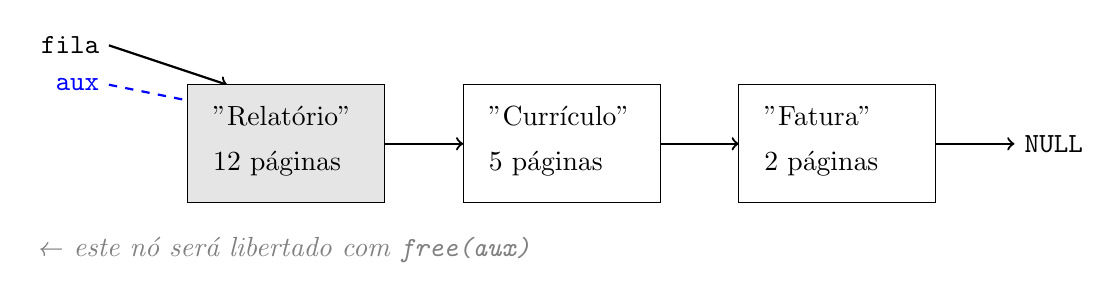
\begin{tikzpicture}

% Setas "fila" e "aux"
\draw[->, thick] (-1, 2) -- (0.5, 1.5);
\node[anchor=east] at (-1, 2) {\texttt{fila}};

\draw[->, thick, dashed, blue] (-1, 1.5) -- (0.5, 1.2);
\node[anchor=east, blue] at (-1, 1.5) {\texttt{aux}};

% Nó 1 (a ser removido)
\draw[fill=gray!20] (0, 0) rectangle (2.5, 1.5);
\node[anchor=west] at (0.2, 1.1) {"Relatório"};
\node[anchor=west] at (0.2, 0.5) {12 páginas};

% Seta para nó 2
\draw[->, thick] (2.5, 0.75) -- ++(1, 0);

% Nó 2 (novo início da fila)
\draw (3.5, 0) rectangle (6, 1.5);
\node[anchor=west] at (3.7, 1.1) {"Currículo"};
\node[anchor=west] at (3.7, 0.5) {5 páginas};

% Seta para nó 3
\draw[->, thick] (6, 0.75) -- ++(1, 0);

% Nó 3
\draw (7, 0) rectangle (9.5, 1.5);
\node[anchor=west] at (7.2, 1.1) {"Fatura"};
\node[anchor=west] at (7.2, 0.5) {2 páginas};

% Última seta para NULL
\draw[->, thick] (9.5, 0.75) -- ++(1, 0);
\node at (11, 0.75) {\texttt{NULL}};

% Legenda
\node[gray] at (1.25, -0.6) {\textit{← este nó será libertado com \texttt{free(aux)}}};

\end{tikzpicture}
\end{center}

\end{document}
